\begin{figure}[htbp]
    \captionsetup[subfigure]{justification=centering}
    \centering
    \begin{subfigure}[b]{0.3\textwidth}
        \centering
        %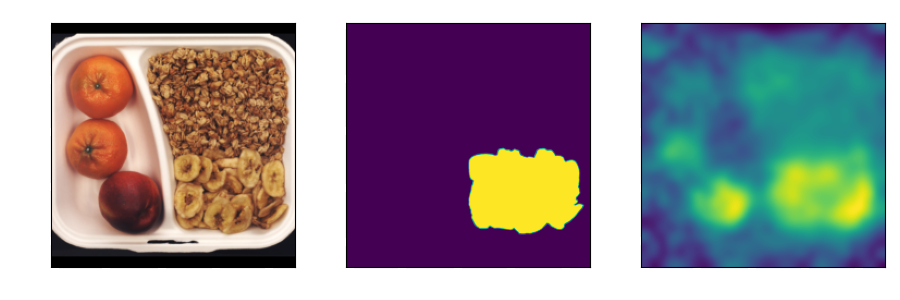
\includegraphics[width=\textwidth]{figures/locopatchcoreresults/breakfast_box_test_logical_anomalies_003.png}
        %\caption*{Logical Anomalies}

    \end{subfigure}
    \begin{subfigure}[b]{0.3\textwidth}
        \centering
        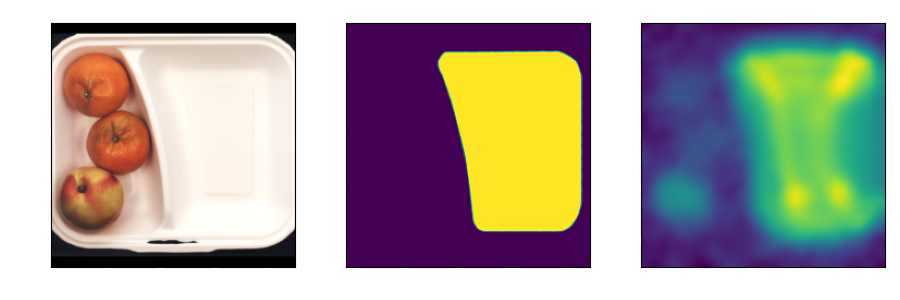
\includegraphics[width=\textwidth]{figures/locopatchcoreresults/breakfast_box_test_logical_anomalies_034.png}


    \end{subfigure}
    \begin{subfigure}[b]{0.3\textwidth}
        \centering
        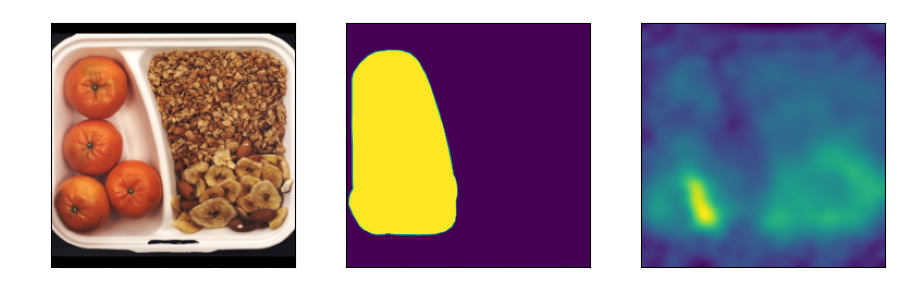
\includegraphics[width=\textwidth]{figures/locopatchcoreresults/breakfast_box_test_logical_anomalies_070.png}


    \end{subfigure}
    \begin{subfigure}[b]{0.3\textwidth}
        \centering
        %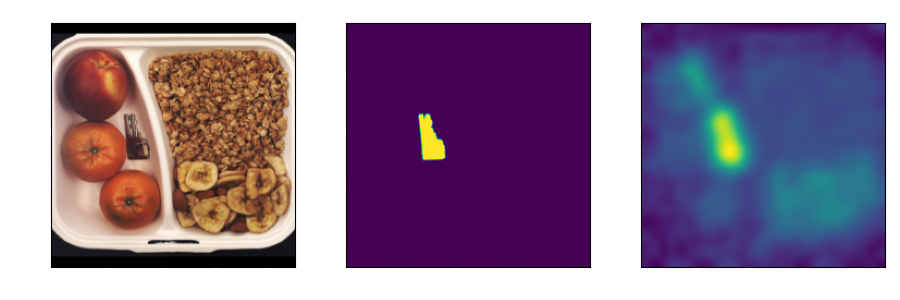
\includegraphics[width=\textwidth]{figures/locopatchcoreresults/breakfast_box_test_structural_anomalies_014.png}
        %\caption*{Structural Anomalies}

    \end{subfigure}
    \begin{subfigure}[b]{0.3\textwidth}
        \centering
        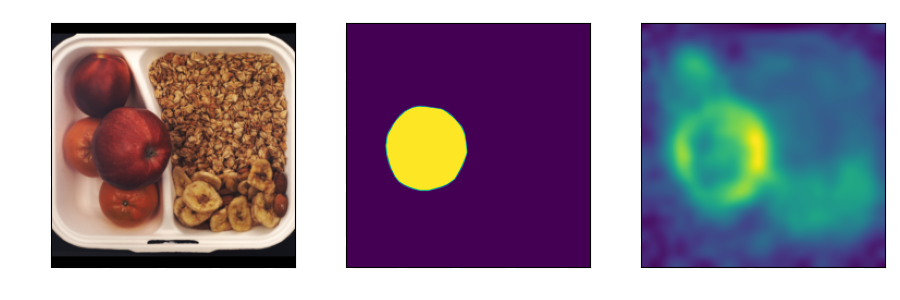
\includegraphics[width=\textwidth]{figures/locopatchcoreresults/breakfast_box_test_structural_anomalies_024.png}


    \end{subfigure}
    \begin{subfigure}[b]{0.3\textwidth}
        \centering
        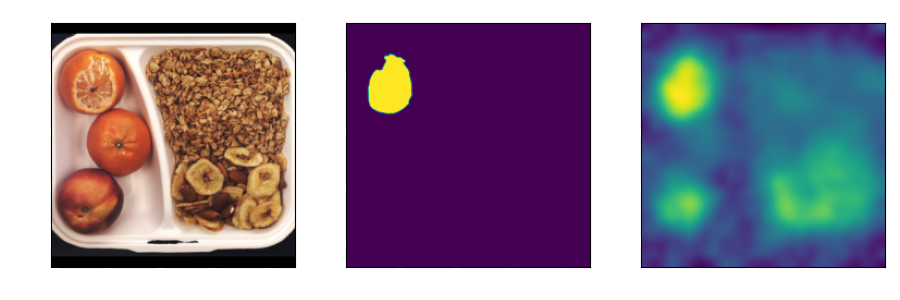
\includegraphics[width=\textwidth]{figures/locopatchcoreresults/breakfast_box_test_structural_anomalies_070.png}


    \end{subfigure}
    \caption{Representative segmentation results from PatchCore \cite{patchCore2022} on the breakfast box class of the MVTecAD LOCO \cite{LOCODentsAndScratchesBergmann2022} dataset.}
    \label{fig:PCBB}
\end{figure}